\chapter{Evaporation-induced pumping of an atom laser}
\label{KineticTheory}
\graphicspath{{Figures/KineticTheory/}{Figures/Common/}}

The pumping process of an atom laser --- just like that of an photon laser --- is a necessarily irreversible process. This irreversibility enters through the coupling of the lasing mode to a much larger system (the reservoir).  For the photon laser this is comprised of the (almost) empty modes of the optical field that the atoms decay into after emitting a photon into the lasing mode (see \sectionref{Introduction:ThePumpingMechanism}).  In the case of the atom laser, there are two possible choices for the reservoir providing the irreversibility: empty modes of an optical field, or empty modes of an atomic field.  The former case was considered in the previous chapter, the latter is the subject of this chapter. 

% The results presented in this chapter have been submitted for publication\footnote{FIXME: Not yet true, but it is intended that this be the case.}.  
The results and analysis presented in \sectionref{KineticTheory:Results} of this chapter was my own work.  The model presented in \sectionref{KineticTheory:Model} is based on prior work~\citep{Davis:2000vn,Bijlsma:2000}.  The derivation of the three-body loss term in \sectionref{MethodsAppendix:QKT3BodyLoss} and the code the results in this chapter are based on are the work of \emph{Matthew Davis}.

\section{Introduction}

Continuous pumping of an atom laser is a key tool for producing superior atomic sources. Besides the obvious benefit of higher flux, it also promises improved modal stability \citep{Haine:2002kp,Haine:2003fs} and linewidth \citep{Johnsson:2007}, much as it does for the photon laser.

There are two essential steps towards the continuous pumping of an atom laser. The first is a delivery system for filling an atomic reservoir with ultracold atoms. The second is a process that causes at least some of those atoms to make an irreversible, atom-stimulated transition into the BEC.

Continuous delivery of ultracold atoms has been demonstrated in a number of experiments \citep{Schmid:2006,Lahaye:2004,Greiner:2001,Greiner:2007,Streed:2006,Muller:2007}, and is an important component of thermal atomic interferometry experiments.  The atom-stimulated transitions into the condensate can be made irreversible by coupling to a reservoir. In this chapter we consider the case in which the reservoir is comprised of empty modes of the atomic field accessible via evaporation.

Sequential reloading of a target BEC was achieved using optical tweezers~\citep{Chikkatur:2002qa}, where a series of source condensates were added adiabatically by manipulating the trapping potentials, and excitations were subsequently removed by continuous evaporation. This milestone experiment maintained the condensate fraction, and therefore the flux of a potential atom laser. An atom laser produced from such an experiment would, however, not possess the desired narrow linewidth as the source condensates used were of a similar size to or larger than the condensate being replenished causing significant scattering into modes other than the target condensate. To produce an atom laser with a narrow linewidth it would be necessary for the atomic source to negligibly disrupt the target condensate.  While this could be achieved by merging the target condensate with significantly smaller condensates more frequently, it is technically very challenging to develop high flux sources of Bose-condensed atoms compared to sources at higher temperature, which have a higher average flux. In this chapter it is shown that a similar experiment using an ultra-cold \emph{thermal} source ought to be able to pump the target BEC and maintain a significant BEC population using a phase-preserving Bose-enhanced process.

%This method has the advantage that it can be performed without the presence of resonant light, but the obvious disadvantage that it relies on the system approaching thermal equilibrium, and will therefore be reversed by the addition of atoms above the condensate temperature. In this chapter it is demonstrated that a driven system undergoing evaporative cooling can produce a high-flux, phase-stable atom laser for a range of experimental parameters.

% FIXME: Something about the fact that one of the distinguishing aspects of this work is the inclusion of three-body loss, as it has been omitted in previous models. While that may be adequate for treatments of the process of condensation, it is inadequate for any treatment of the creation of a pumped atom laser (as will be later argued).

\section{Scheme}
\label{KineticTheory:Scheme}

\begin{figure}
    \centering
        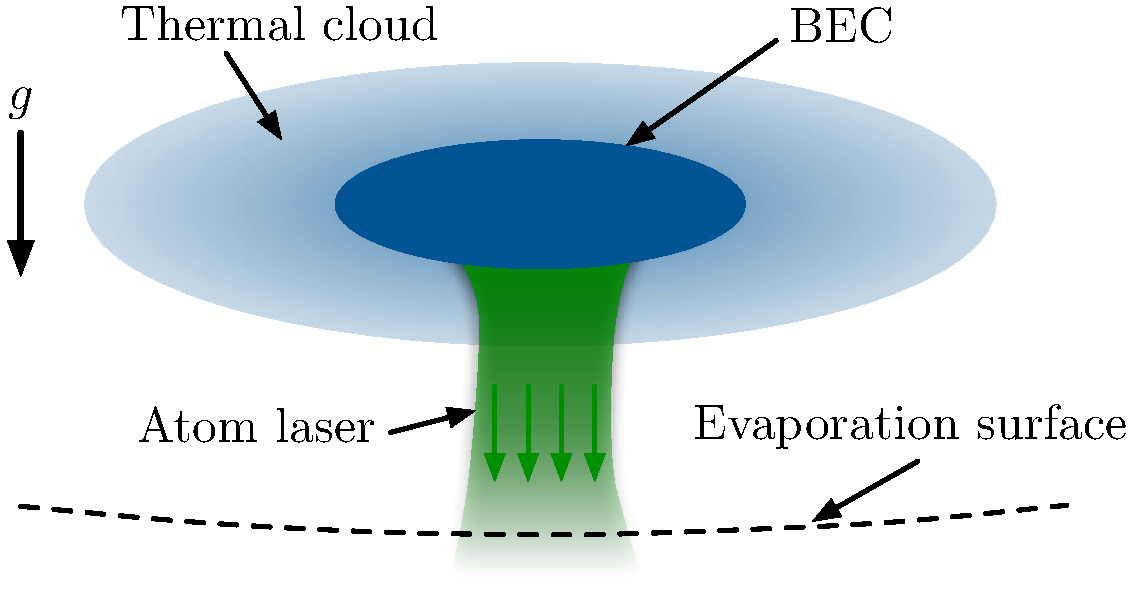
\includegraphics[width=10cm]{QKTScheme}
    \caption{Schematic of the experimental setup.}
    \label{KineticTheory:QKTScheme}
\end{figure}

The proposed scheme for a pumped atom laser is illustrated in \figureref{KineticTheory:QKTScheme} and is very similar to the processes used to evaporate a thermal cloud to condensation in a magnetic trap and produce a (quasi-continuous) atom laser. The additional element in this scheme is a process for replenishing the cloud of thermal atoms in the trap.  

In this scheme the gain process for the condensate is the same Bose-enhanced scattering process between thermal atoms and the condensate that drives condensate growth when evaporating to produce BEC~\citep{Gardiner:1997kx,Davis:2000vn,Bijlsma:2000}.  This process becomes irreversible when one of the scattered atoms has enough energy to cross the evaporation surface and be removed from the thermal cloud.  The loss of atoms from the thermal cloud is balanced by a replenishment process that couples the thermal cloud to a source of atoms at finite temperature.

The atom laser beam itself is produced by outcoupling from the condensate.  To minimise direct outcoupling from the thermal cloud, this outcoupling process should be a large momentum-transfer Raman process to limit the range of momenta of thermal particles that will be outcoupled.  Outcoupling of thermal atoms can be reduced further by focussing the Raman lasers to only intersect in the immediate vicinity of the condensate.

A dynamic equilibrium will be reached when the rate of atom loss from the condensate due to outcoupling balances the rate of atoms gained due to scattering with the thermal cloud.  If the evaporative surface is tuned so that atoms of energy $\varepsilon_\text{cut}$ and higher are rapidly and continually removed from the trap, then all collisions that give atoms energy greater than $\varepsilon_\text{cut}$ will become irreversible. As $\varepsilon_\text{cut}$ is lowered, a larger fraction of the scattering processes that leave atoms in the condensate mode will become irreversible. This suggests that there must be some value of $\varepsilon_\text{cut}$ for which the condensate experiences net gain. What is not clear is whether the net gain can proceed efficiently, i.e.\ on a timescale much shorter than other losses from the condensate.  Lowering $\varepsilon_\text{cut}$ also reduces the total number of thermal atoms present. In the limit that $\varepsilon_\text{cut}$ reaches the condensate energy, there will be no background gas at all, and the condensate cannot experience net gain.  We therefore expect that for a given set of parameters, there will be an optimal value for $\varepsilon_\text{cut}$ that maximises the net gain, which may or may not be positive. In order to examine this issue, quantum kinetic theory (QKT)~\citep{Gardiner:1997tz,Jaksch:1997ug,Gardiner:1998wx,Jaksch:1998sj,Gardiner:2000ug,Lee:2000vs,Davis:2000vn} has been employed, which has been effective in describing the growth of condensates~\citep{Davis:2000vn}.


\section{Model}
\label{KineticTheory:Model}

\begin{figure}
    \centering
        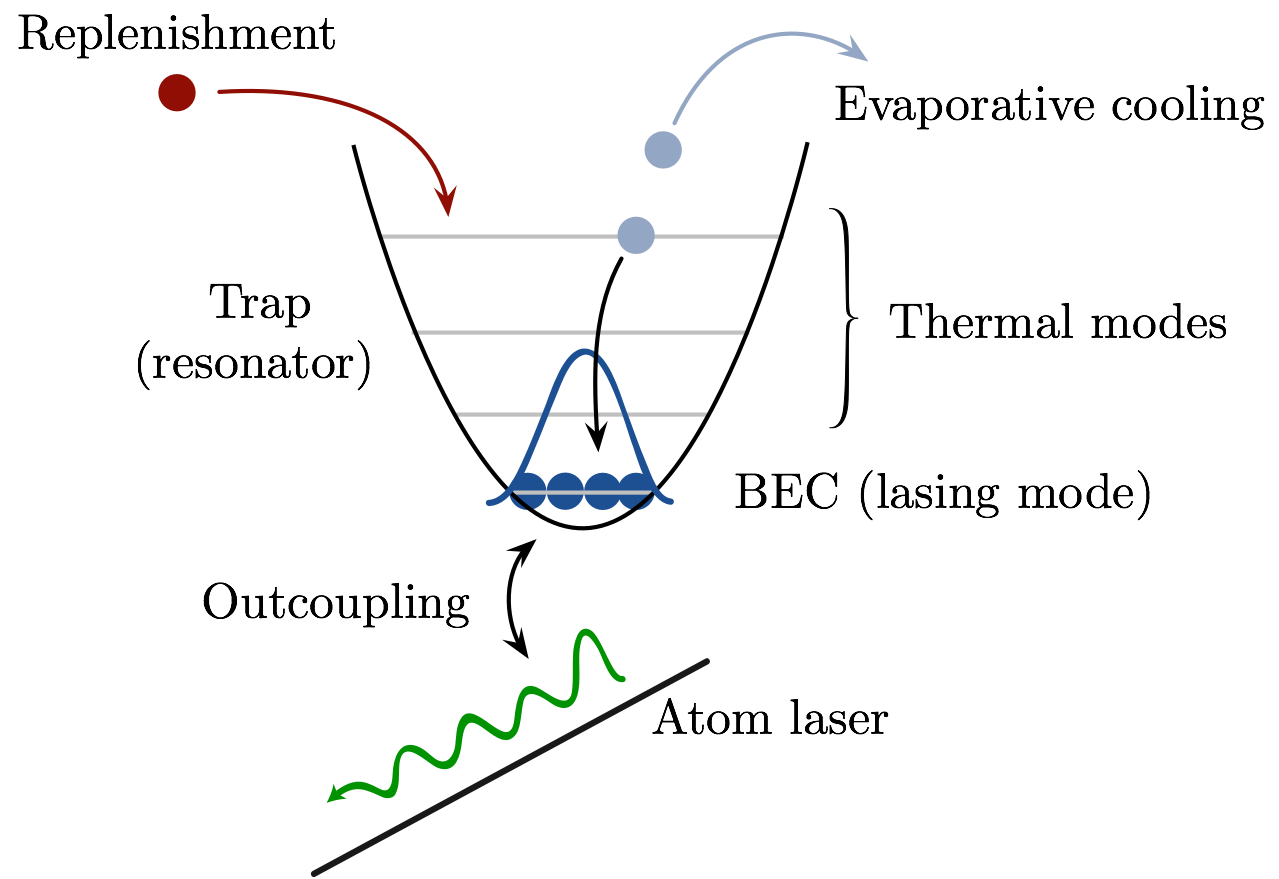
\includegraphics[width=10cm]{QKTModel2}
    \caption{Schematic of the theoretical model.}
    \label{KineticTheory:QKTModel}
\end{figure}

The theoretical model described in this section is an extension of the kinetic model of~\citet{Bijlsma:2000}, which was successfully used to study condensate growth in an experiment in which a cloud of thermal atoms just above condensation temperature were shock-cooled below transition~\citep{Miesner:1998}.  After shock-cooling, the atoms were left to equilibrate, with condensate formation being driven by the same collisional processes that would drive condensate growth in the proposed pumped atom laser experiment described in the previous section.  To fully describe this proposed experiment, the kinetic model of~\citeauthor{Bijlsma:2000} must be modified to include the effects of the replenishment and outcoupling processes illustrated in \figureref{KineticTheory:QKTScheme}. 

Another important process that must be included in the model is three-body recombination, which is the dominant loss process in typical BEC experiments~\citep{Burt:1997fk,Soding:1999}. Without the inclusion of this process, for given replenishment and outcoupling rates, the largest condensate would be formed in the absence of evaporation as outcoupling from the condensate would be the only loss process in the system. In fact, this condensate number would be independent of the temperature of the replenishment source, depending only on the flux of atoms delivered to the system and the outcoupling rate from the condensate. This unphysical result is because in the absence of a density-dependent loss process, simply increasing the density is a feasible method of approaching degeneracy. It would be possible to reach condensation with room-temperature atoms in a harmonic trap simply by confining enough atoms! To avoid such unphysical results, the effect of three-body loss as the dominant density-dependent loss process must be included in the model.

\parasep

The starting point of the kinetic model presented here is to treat separately the thermal and condensed components of the system in \figureref{KineticTheory:QKTScheme}.

The condensed component is assumed to be a quantum fluid obeying a Gross-Pitaevskii-type equation, however we make a further approximation and assume that the condensate is sufficiently occupied that it has a Thomas-Fermi profile.  The condensate dynamics are then fully described by the number of condensed atoms $N_0(t)$.

The thermal cloud is assumed to be well described within the Hartree-Fock approximation~\citep[Chapter 8]{PethickSmith} as comprised of particle-like excitations moving in the effective potential of the harmonic trap plus condensate mean field.  To reduce the dimensionality of the full phase-space distribution function for the thermal cloud $f(\vect{r}, \vect{p}, t)$, it is assumed that the system is ergodic, i.e.\  that all points in the phase space having the same energy are equally probable.  Under this approximation, the thermal cloud is then described by its energy distribution function $g(\varepsilon, t)$ and the density of states $\rho(\varepsilon, t)$.  The assumption of ergodicity has been shown in the past to give good agreement with experiment when asymmetric spatial or momentum dynamics are not significant~\citep{Bijlsma:2000,Davis:2000vn}.  Note that the time-dependence of the density of states $\rho(\varepsilon, t)$ comes from the contribution of the condensate mean field to the effective potential experienced by the thermal atoms.


As the model presented here is very similar to that presented in~\citep{Bijlsma:2000} with some additional terms, a derivation of the common terms is omitted. As a summary, the derivation proceeds by taking a semiclassical Boltzmann equation for the phase-space distribution function of the thermal cloud $f(\vect{r}, \vect{p}, t)$ including collisional terms and using the ergodic approximation to obtain an equation of motion for the energy distribution function $g(\varepsilon, t)$. This equation is self-consistently matched with a Gross-Pitaevskii equation for the condensate before making the Thomas-Fermi approximation to obtain an equation of motion for the number of condensed atoms $N_0(t)$. An example application of this method to derive the appropriate terms for three-body loss is given in \sectionref{MethodsAppendix:QKT3BodyLoss}. Further, a detailed discussion of this theory is given in the review article~\citep{Proukakis:2008}.

Separating the contributions of the different processes involved, the equations of motion for the model for a collision-driven pumped atom laser considered here are
\begin{align}
    \frac{d N_0}{d t} =\begin{split}
        &\relphantom{+}\left. \frac{d N_0}{d t}\right|_\text{thermal--condensate} \\
        &+\left. \frac{d N_0}{d t}\right|_\text{3-body loss} \\
        &+\left. \frac{d N_0}{d t}\right|_\text{outcoupling}
    \end{split},
    & \frac{\partial (\rho g)}{\partial t} = \begin{split}
        &\relphantom{+}\left. \frac{\partial (\rho g)}{\partial t}\right|_\text{thermal--thermal} \\
        &+\left. \frac{\partial (\rho g)}{\partial t}\right|_\text{thermal--condensate} \\
        &+\left. \frac{\partial (\rho g)}{\partial t}\right|_\text{3-body loss} \\
        &+\left. \frac{\partial (\rho g)}{\partial t}\right|_\text{replenishment} \\
        &+\left. \frac{\partial (\rho g)}{\partial t}\right|_\text{redistribution}
    \end{split},
    \label{KineticTheory:EvolutionEquations}
\end{align}
where the subscripts `thermal--thermal' and `thermal--condensate' denote Bose-enhanced collisional processes between atoms in the corresponding states [\figureref{KineticTheory:ProcessDiagrams}(a) and (b), respectively], the subscript `3-body loss' indicates the contribution due to three-body recombination [\figureref{KineticTheory:ProcessDiagrams}(f)], the subscript `replenishment' indicates the contribution due to the replenishment of the thermal cloud [\figureref{KineticTheory:ProcessDiagrams}(d)], the subscript `outcoupling' indicates the contribution due to outcoupling from the condensate to form the atom laser [\figureref{KineticTheory:ProcessDiagrams}(e)], and the subscript `redistribution' indicates the contribution due to the redistribution of population in energy space due to the changes of the energies of the occupied levels as the mean-field of the condensate changes [\figureref{KineticTheory:ProcessDiagrams}(c)]. It is assumed that atoms with energy greater than the evaporative energy cut-off $\varepsilon_\text{cut}$ are removed from the system sufficiently quickly that  $g(\varepsilon > \varepsilon_\text{cut}) = 0$.

\begin{figure}
    \centering
    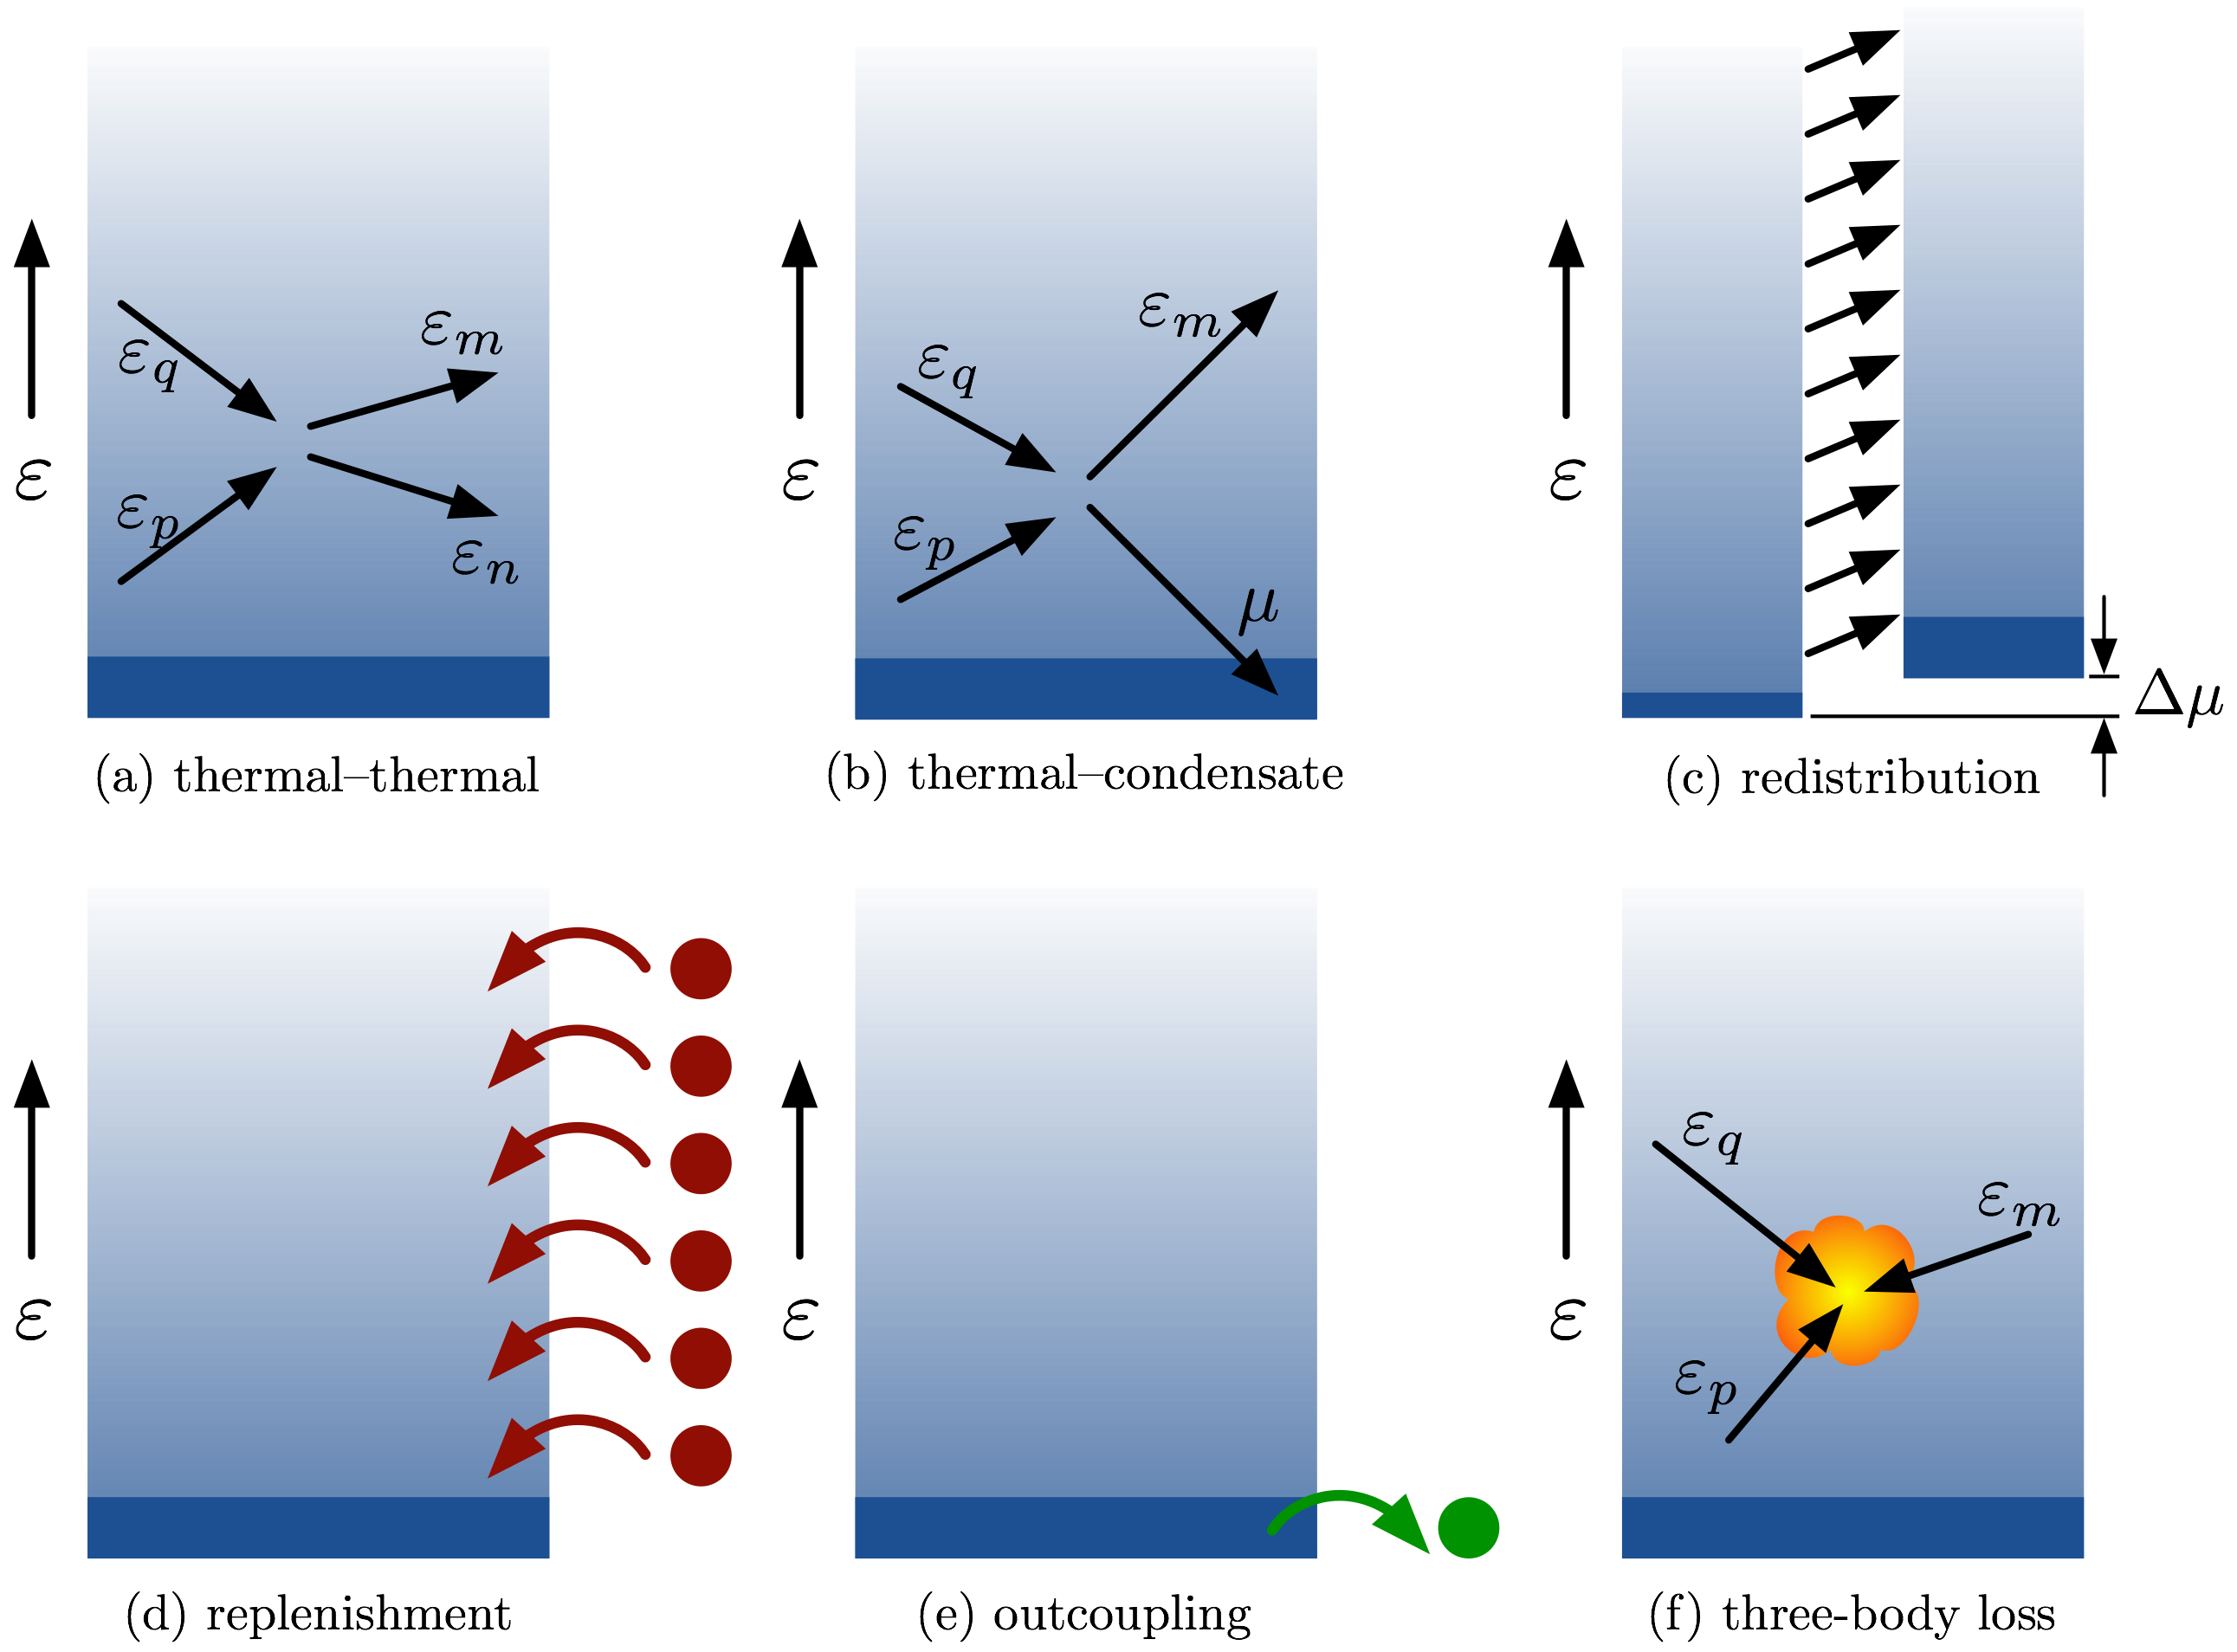
\includegraphics[width=14cm]{ProcessDiagrams}
    \caption{Schematic of processes involved in the evolution of the kinetic model described by \eqref{KineticTheory:EvolutionEquations}.  The upper shaded rectangle in each subfigure represents the energy distribution function $g(\varepsilon, t)$ of the thermal cloud, and the bottom dark blue rectangle represents the condensate with occupancy $N_0(t)$ and energy $\varepsilon = \mu(t)$. Figures (a) and (b) represent collisional processes involving two thermal atoms and one thermal and one condensate atom respectively. Figure (c) represents the change in the energy distribution function $g(\varepsilon, t)$ if the condensate occupation (and hence chemical potential) changes, changing the energies of every energy level. Figure (d) represents the replenishment of the thermal cloud from an atomic reservoir, Figure (e) represents outcoupling from the condensate mode to produce the atom laser, and Figure (f) represents the loss of atoms due to three-body recombination.}
    \label{KineticTheory:ProcessDiagrams}
\end{figure}

The forms of the `thermal--thermal', `thermal--condensate' and `redistribution' terms in \eqref{KineticTheory:EvolutionEquations} are given in \sectionref{MethodsAppendix:QKTOtherTerms} and derivations are given in~\citep{Bijlsma:2000}.

The outcoupling process from the condensate is modelled as a simple linear loss process with corresponding rate constant $\gamma$,
\begin{align}
    \left.\frac{d N_0}{d t}\right|_\text{outcoupling} &= - \gamma N_0.
    \label{KineticTheory:OutcouplingProcess}
\end{align}
In modelling the outcoupling in this way, any outcoupling from thermal modes has been neglected. As discussed in \sectionref{KineticTheory:Scheme}, this is a reasonable approximation if focused Raman lasers are used for the outcoupling which only intersect in the immediate vicinity of the condensate. 

The thermal cloud is modelled as being continuously replenished from a source that provides a constant flux $\Phi$ of atoms at a temperature $T$.  To avoid tying the model to any particular replenishment mechanism, we assume a best-case scenario in which each energy level $\varepsilon$ in the source is coupled directly to the level in the thermal cloud with the same energy above the condensate chemical potential $\mu(t)$, i.e.\ the lowest energy level of the source ($\varepsilon=0$) is coupled directly to the lowest energy level in the trap ($\varepsilon = \mu(t)$).  This simple model gives the form of the contribution due to replenishment as
\begin{align}
    \left. \frac{\partial \big(\rho(\varepsilon, t) g(\varepsilon, t)\big)}{\partial t} \right|_\text{replenishment} &= \Gamma \rho_0(\varepsilon - \mu(t)) g_T(\varepsilon - \mu(t)),
    \label{KineticTheory:ReplenishmentProcess}
\end{align}
where $\rho_0(\varepsilon)$ is the density of states in the absence of a condensate, $g_T(\varepsilon)$ is the Bose-Einstein  distribution at temperature $T$, and $\Gamma$ is a rate constant such that
\begin{align}
    \Gamma \int_0^\infty \rho_0(\varepsilon) g_T(\varepsilon)\, d\varepsilon = \Phi,
    \label{KineticTheory:GammaPhiRelation}
\end{align}
where $\Phi$ is the flux of atoms from the source \emph{before} evaporation.  The derivation of the contributions to \eqref{KineticTheory:EvolutionEquations} due to three body loss were performed by \emph{Matthew Davis}, and are given in \sectionref{MethodsAppendix:QKT3BodyLoss}.
%While this is perhaps an unreasonable assumption, it means that we can easily determine the steady state of the system.

\parasep

We summarise here the approximations made in obtaining the kinetic model \eqref{KineticTheory:EvolutionEquations}:
\begin{enumerate}[(i)]
    \item The energy scale of the thermal cloud is large enough that all excitations are particle-like and not collective excitations such as phonons. Phonon-like excitations are only important for particle energies $\varepsilon \lesssim 2\mu(t)$~\citep[\S 8.3.1]{PethickSmith}. Hence, we require that the energy scale for the thermal cloud $\varepsilon_\text{cut}$ be much larger than $\mu(t)$.
    \item The phase-space distribution of the thermal cloud is ergodic and hence is purely a function of energy. This assumption is true at equilibrium, however it needs some justification when used in non-equilibrium scenarios. In this case, asymmetric behaviour of the condensate is not expected in either position or momentum space 
    \item The condensate density is sufficiently large that it is well-described by a Thomas-Fermi profile. This approximation is justified as it is only the large-condensate limit that is of interest as a large condensate will be necessary for the production of a high-flux atom laser in this scheme. In making this approximation, the effects of both the normal and anomalous densities of the thermal cloud on the condensate have also been neglected.
    \item Evaporation occurs on a time-scale faster than collisions. This is the usual requirement during evaporation to condensation, and so should be satisfied in the proposed experiment.
\end{enumerate}

The computer code used to solve the kinetic model \eqref{KineticTheory:EvolutionEquations} was written by \emph{Matthew Davis}.  This code is a modified version of that used in \citep{Davis:2000vn}, which has shown good agreement with an independently created code by \citet{Bijlsma:2000}.  The results and analysis presented in the remainder of this chapter are my own work.

\section{Simulation results}
\label{KineticTheory:Results}

For a given trap geometry, the model is fully defined by the flux of replenishment atoms $\Phi$, the temperature $T$ of those atoms, the energy of the evaporative cut $\varepsilon_\text{cut}$, and the outcoupling rate from the condensate $\gamma$. In this section the results of the kinetic model for some `typical' parameter values are presented, and the dependence of the model on each of the parameters is examined.

Our numerical simulations are based on a trap and conditions similar to that of~\citep{Kohl:2002}, who precooled a cloud of $\nucl{87}{Rb}$ atoms to an initial temperature slightly greater than the critical temperature before performing evaporative cooling to study condensate growth.  The trap in the experiment was axially-symmetric with radial and axial trapping frequencies of  $\omega_r = \unit[2 \pi \times 110]{Hz}$ and $\omega_z = \unit[2\pi \times 14]{Hz}$ respectively.

To numerically solve the kinetic model, \eqref{KineticTheory:EvolutionEquations} is discretised along the energy dimension and the resulting coupled differential equations are solved with an adaptive fourth-fifth Runge-Kutta~\citep{NumericalRecipes} method. Our results are mainly concerned with the steady-state of the kinetic model, which we define as being reached when the condensate number has changed by less than either $0.1\%$ or $1$ atom in $\unit[100]{ms}$.  The initial state for the simulation is chosen to be a truncated Bose-Einstein distribution containing (before truncation) $N_\text{initial} = \unit[4.2\times 10^6]{atoms}$ at the same temperature as the replenishment reservoir.  This state is chosen as a representation of the steady-state of the system prior to evaporation.  In the trap considered, the critical temperature for $4.2\times 10^6$ atoms is $T_c = \unit[400]{nK}$.


\subsection{Typical dynamics and parameter studies}
\label{KineticTheory:ParameterStudies}

\begin{figure}
    \centering
    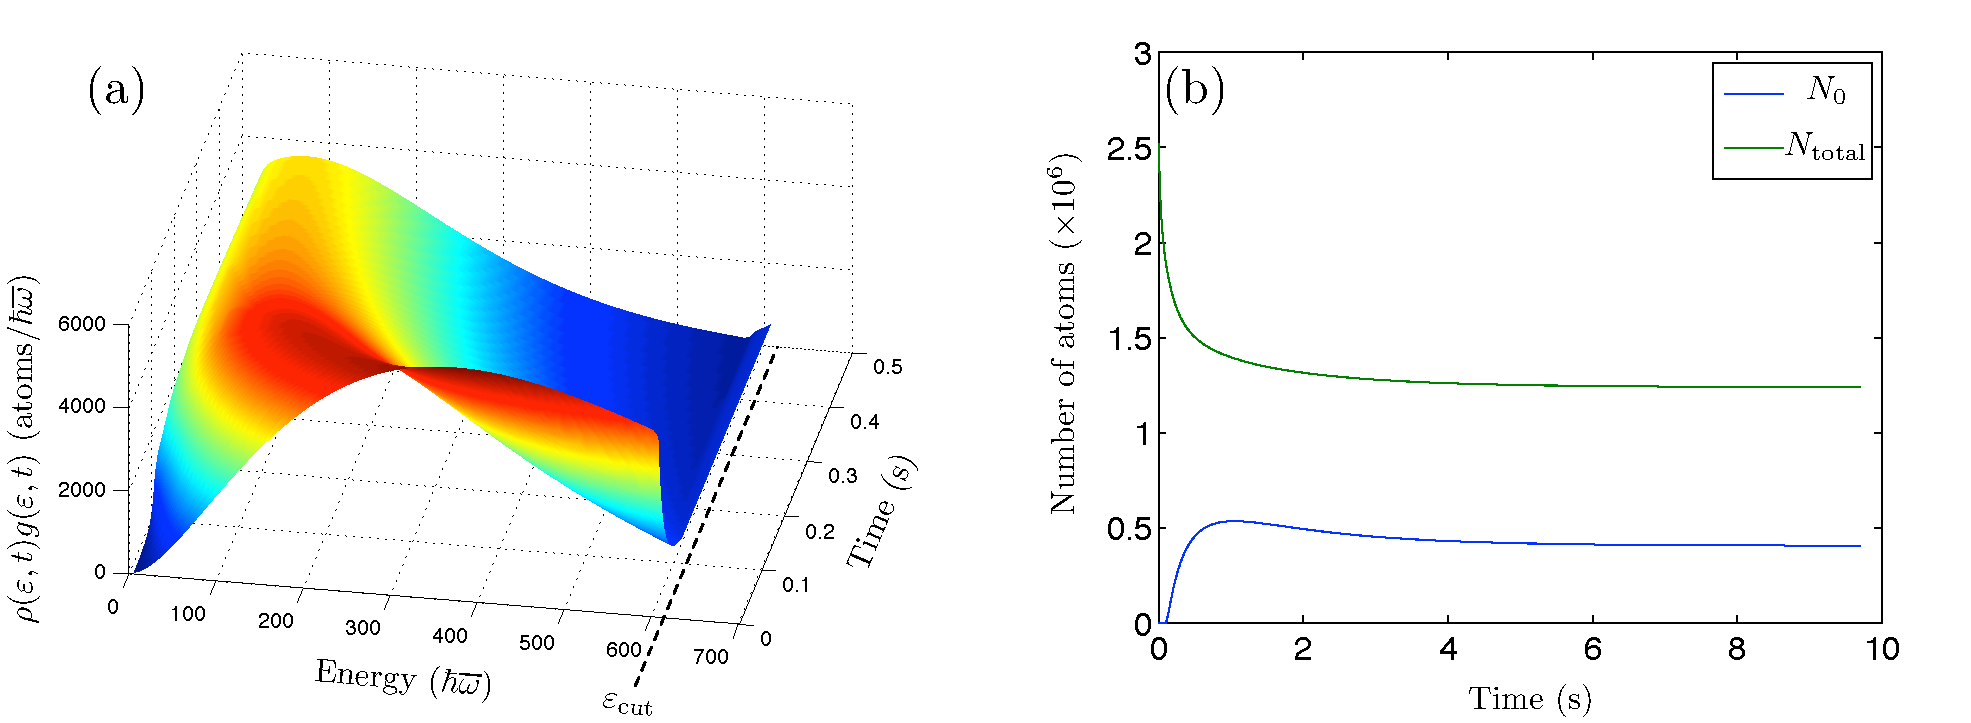
\includegraphics[width=15cm]{EnergyDistributionFunctionEvolution}
    \caption{Results of the kinetic model for $\Phi = \unit[8.4 \times 10^5]{atoms/s}$, $T=\unit[540]{nK}$, $\varepsilon_\text{cut} = 3 k_B T \approx 610 \hbar \overline{\omega}$, and $\gamma = \unit[0.3]{s\textsuperscript{-1}}$. Figure (a) highlights the dynamics of the occupation of the thermal energy levels for $t < \unit[0.5]{s}$, while (b) illustrates the equilibration of the total and condensed atom numbers over $\sim \unit[10]{s}$. The energy distribution at $t=0$ is a truncated Bose-Einstein distribution containing (before truncation) $N=4.2\times 10^6$~atoms at $T=\unit[540]{nK}$.
    }
    \label{KineticTheory:EnergyDistributionFunctionEvolution}
\end{figure}

As a depiction of the `typical' time-dependence of the results obtained from the kinetic theory model \eqref{KineticTheory:EvolutionEquations}, we consider the case of pumping the system continuously with a source such that the initial number $N = 4.2\times 10^6$ is transferred to the system once every 5 seconds giving a flux of $\Phi = \unit[8.4 \times 10^5]{atoms/s}$.  The temperature of the replenishment source is chosen to be $T=\unit[540]{nK}$, 60\% above the condensation temperature of the system before evaporation.  For the remaining model parameters, we choose the evaporative cut-off to be $\varepsilon_\text{cut} = 3 k_B T$, and the outcoupling rate from the condensate to be $\gamma = \unit[0.3]{s\textsuperscript{-1}}$.  

\figureref{KineticTheory:EnergyDistributionFunctionEvolution} illustrates the results of the simulation of this system.  \figureref{KineticTheory:EnergyDistributionFunctionEvolution}(a) shows the energy distribution of the thermal cloud cooling from the initial truncated Bose-Einstein distribution to a distribution with a lower average energy per particle.  \figureref{KineticTheory:EnergyDistributionFunctionEvolution}(b) demonstrates that despite pumping the system with an atomic reservoir above critical temperature that it is possible to reach a steady-state in which the condensate is macroscopically occupied.  In this example, the steady-state condensate fraction is 33\%.

\begin{figure}
    \centering
    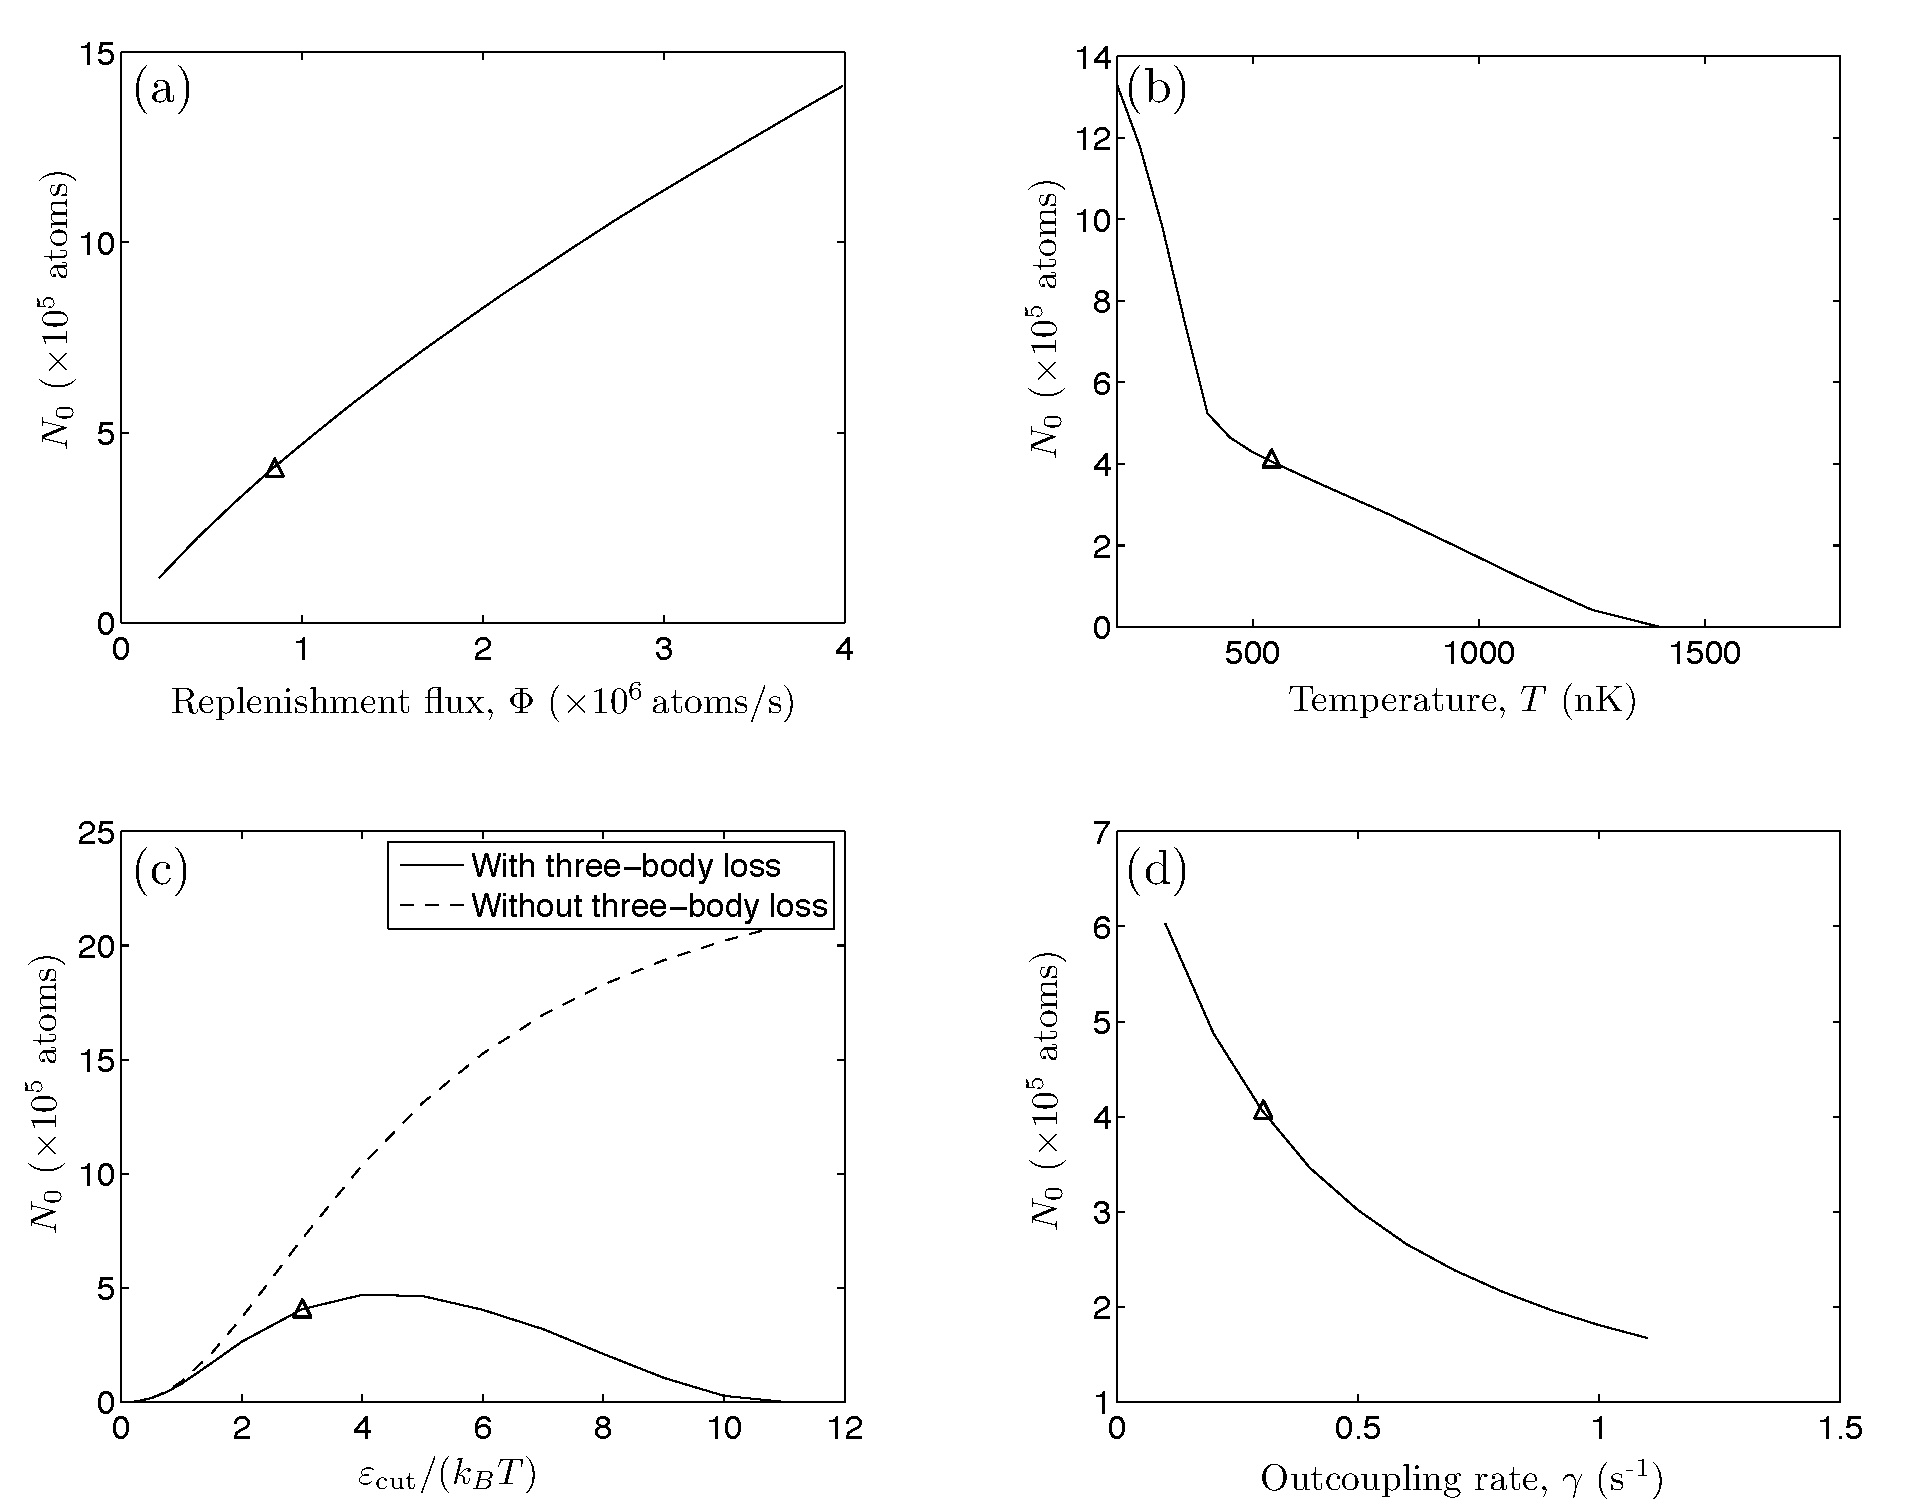
\includegraphics[width=15cm]{ParameterStudies}
    \caption{The dependence of the equilibrium condensate number $N_0$ on the parameters of the quantum kinetic model \eqref{KineticTheory:EvolutionEquations}. The equilibrium condensate number has a monotonic dependence on the replenishment flux (a), the temperature of the replenishment source (b) and the outcoupling rate (d). For a given choice of the remaining parameters of the model there is an optimum $\varepsilon_\text{cut}$ (c) for which the equilibrium condensate number is a maximum. For each parameter being varied, the remaining parameters are chosen to be the same as for the results depicted in \figureref{KineticTheory:EnergyDistributionFunctionEvolution}. The triangle in each plot marks the point that corresponds to the precise conditions of \figureref{KineticTheory:EnergyDistributionFunctionEvolution}.}
    \label{KineticTheory:ParameterStudies}
\end{figure}

The details of the equilibration of the system are not the subject of investigation here, instead our interest is in the equilibrium itself, and in determining the feasibility of creating a pumped atom laser driven by a non-condensed atomic source.  As a first step towards this investigation we consider the dependence of the equilibrium condensate number on the parameters of the system: $\Phi$, $T$, $\varepsilon_\text{cut}$, and $\gamma$.  The results of such a parameter study are presented in \figureref{KineticTheory:ParameterStudies} in which the dependence on these parameters of the steady-state of the results of \figureref{KineticTheory:EnergyDistributionFunctionEvolution} is investigated.

The majority of the parameter dependences depicted in \figureref{KineticTheory:ParameterStudies} are trivial; increasing the relevant parameter causes a monotonic change in the equilibrium condensate number.  Increasing the flux of atoms to the system increases the equilibrium condensate number [\figureref{KineticTheory:ParameterStudies}(a)], while increasing the temperature of the replenishment source or increasing the outcoupling rate reduces the equilibrium condensate number [\figureref{KineticTheory:ParameterStudies}(b) and \figureref{KineticTheory:ParameterStudies}(d) respectively].  The sharp kink in \figureref{KineticTheory:ParameterStudies}(b) occurs exactly at $T=T_c$ and is due to condensation of the source cloud.  The only non-trivial behaviour is displayed by \figureref{KineticTheory:ParameterStudies}(c) in which the dependence on the evaporative cut-off $\varepsilon_\text{cut}$ is illustrated.  For large evaporative cut-offs, few atoms will be lost due to evaporation and the system will reach equilibrium when the flux of atoms into the system is balanced by three-body losses and outcoupling from the condensate.  As $\varepsilon_\text{cut}$ is reduced, more atoms are lost due to evaporation and the mean energy per particle reduces, causing the condensate size to increase.  As $\varepsilon_\text{cut}$ continues to reduce, an increasing fraction of the replenishment atoms have an energy greater than $\varepsilon_\text{cut}$, causing a lower effective atomic flux to be delivered to the system. This reduces the potential size of any condensate formed.  These two competing effects are the origin of the existence of an optimum equilibrium condensate number as a function of $\varepsilon_\text{cut}$ in \figureref{KineticTheory:ParameterStudies}(c).

As discussed earlier, in the absence of three-body loss, the equilibrium condensate number would continue to increase as $\varepsilon_\text{cut}$ is increased, which would lead to the unphysical conclusion that evaporating \emph{reduces} the equilibrium condensate number.  This is demonstrated by the dashed line in \figureref{KineticTheory:ParameterStudies}(c) which asymptotes towards $N_0=\Phi/\gamma = \unit[2.8\times 10^6]{atoms}$ in the limit $\varepsilon_\text{cut}\rightarrow \infty$.  As observed in the remaining panels of \figureref{KineticTheory:ParameterStudies} (in which the effects of three-body loss have been included) three-body loss does not give rise to optimum values for the corresponding parameters of the model as it is only changes to $\varepsilon_\text{cut}$ that affect the evaporative and three-body losses in contrary fashions.  An increase in the replenishment flux will increase both evaporative and three-body losses.  Similarly, changes to the temperature of the replenishment source or the outcoupling rate either increase both or decrease both of the evaporative and three-body losses.

At this point the fairly obvious recommendation could be made that to have the largest equilibrium condensate number one should use a replenishment source with the highest possible flux and the lowest possible temperature.  It is an experimental reality, however, that these parameters are not orthogonal; while a $\unit[300]{K}$ oven might produce a significantly larger flux than a $\unit[50]{mK}$ 2D-MOT, it is simply not realistic to create a $\unit[50]{mK}$ atomic source with the same flux as the $\unit[300]{K}$ oven.  It is this trade-off between the temperature and flux in the context of experimentally-realisable sources that is the subject of the remainder of the chapter.

%The replenishment process could be treated in a best-case scenario in two different ways: coupling each energy levels directly that have the same energy, or coupling the nth level in one system to the nth level in the other system. The first case corresponds to rapidly combining the systems on a timescale short enough that neither system has time to react; the second case corresponds to the opposite limit in which the systems are coupled slowly enough that each energy level undergoes an adiabatic change towards the corresponding level in the other system.

% We still need more thermal sources for the high-temperature limit part of the text.


\subsection{Behaviour in the high-temperature limit}
In the previous section, the dependence of the equilibrium condensate number on the model parameters was investigated. The physical question that we desire to address with this model is what are the requirements on the replenishment source to produce a pumped atom laser?

Although it would be possible to create a pumped atom laser by combining condensates in a manner similar to the experiment by~\citet{Chikkatur:2002qa}, such an atom laser would have significantly reduced phase-stability unless the replenishment process were essentially continuous. However, to replenish a condensate by collisional interactions with a continuous source of condensed atoms, the replenishment source would itself need to have many of the desired properties of a pumped atom laser! Instead, it is necessary to be able to use a source \emph{above} condensation temperature for replenishment.

We consider now the experimentally-relevant limit of replenishing the thermal cloud using a high-flux source of thermal atoms. For such sources two simplifications are possible. First, for temperatures greater than $T_c$ the Bose-Einstein energy distribution of the source $g_T(\varepsilon)$ is well approximated by the Boltzmann distribution $g_T(\varepsilon) \approx \zeta e^{-\beta \varepsilon}$ for some constant $\zeta$, and $\beta = \left(k_B T\right)^{-1}$. Secondly, for high temperature sources the optimum evaporation cut-off $\varepsilon_\text{cut}$ will be much smaller than the characteristic energy of the source $k_B T$, and hence $\varepsilon_\text{cut} \ll k_B T$.  From these simplifications it can be seen that the energy distribution below the evaporation cut-off is well described by the single parameter $\zeta$ as $g_T(\varepsilon \leq \varepsilon_\text{cut}) \approx \zeta$.

At this point, no overall simplification has occurred as we have simply rewritten the temperature dependence of the replenishment source in terms of the parameter $\zeta$.  However, as the energy distribution of the replenishment source only affects the kinetic model through \eqref{KineticTheory:ReplenishmentProcess}, its influence on the system dynamics is only through the combined quantity $\kappa = \Gamma \zeta$. An expression for $\kappa$ directly in terms of relevant experimental quantities can be obtained using the definition \eqref{KineticTheory:GammaPhiRelation},
\begin{align}
    \Phi &= \Gamma \int_0^\infty \rho_0(\varepsilon) g_T(\varepsilon)\, d\varepsilon \notag\\
    &= \Gamma \int_0^\infty \frac{\varepsilon^2}{2 (\hbar \overline{\omega})^3} \zeta e^{-\beta \varepsilon}\, d\varepsilon \notag\\
    &= \Gamma \zeta \frac{1}{2 (\hbar \overline{\omega})^3} \int_0^\infty \varepsilon^2 e^{-\beta \varepsilon}\, d\varepsilon \notag\\
    &= \left(\frac{k_B T}{\hbar \overline{\omega}}\right)^3 \Gamma \zeta\\
    \kappa &\equiv \Gamma \zeta = \Phi \left(\frac{\hbar \overline{\omega}}{k_B T}\right)^3 \label{KineticTheory:KappaDefinition}
\end{align}
where $\overline{\omega} = \left(\omega_x \omega_y \omega_z\right)^{\frac{1}{3}}$ is the geometric mean of the trapping frequencies, and $\displaystyle\rho_0(\varepsilon) = \frac{\varepsilon^2}{2 (\hbar \overline{\omega})^3}$ is the density of states in a harmonic trap in the absence of a condensate~\citep{PethickSmith}.

We term $\kappa$ the \emph{phase-space flux} of the source as it is directly related to the rate at which the phase-space density of the thermal source is delivered.  For a trap of $N$ thermal atoms at temperature $T$, the peak phase-space density $\varpi$ is~\citep[Chapter 2]{PethickSmith}
\begin{align}
    \varpi &= N \left(\frac{\hbar \overline{\omega}}{k_B T} \right)^3.
\end{align}
If these $N$ atoms are delivered over a time $\tau$ providing a flux $\Phi = N/\tau$ the peak phase-space flux is
\begin{align}
    \frac{\varpi}{\tau} &= \frac{N}{\tau}\left(\frac{\hbar \overline{\omega}}{k_B T}\right)^3 = \Phi \left(\frac{\hbar \overline{\omega}}{k_B T}\right)^3 \equiv \kappa.
\end{align}

The phase-space flux $\kappa$ is a figure-of-merit for the thermal source.  It quantifies the qualitative behaviour already known: for the same atomic flux $\Phi$, a source with a lower temperature will result in a larger condensate [\figureref{KineticTheory:ParameterStudies}(b)]; and for the same temperature, a source with a higher atomic flux will also result in a larger condensate [\figureref{KineticTheory:ParameterStudies}(a)].  The phase-space flux also describes exactly how a trade-off between the flux and temperature of the replenishment source will affect the equilibrium condensate number.  If two sources with different fluxes and temperatures have the same value of phase-space flux, then the equilibrium condensate number produced by the two sources will be the same (assuming the high-temperature limit applies to both sources).  Our interest is in determining what values of $\kappa$ are necessary to produce a pumped atom laser, and whether such values are achievable.

For the limit of high-temperature atomic sources, we have reduced the four variables $(\Phi, T, \varepsilon_\text{cut}, \gamma)$ required to define the model \eqref{KineticTheory:EvolutionEquations} down to three $(\kappa, \varepsilon_\text{cut}, \gamma)$. Of these three, our main interest is in the dependence of the system on the properties of the atomic source through $\kappa$. In contrast, the dependence of the equilibrium condensate number on the outcoupling rate $\gamma$ is simple [see \figureref{KineticTheory:ParameterStudies}(d)] and the results would not be expected to change qualitatively with $\gamma$. It is therefore appropriate to choose a representative value for the outcoupling rate (here $\gamma = \unit[0.3]{s\textsuperscript{-1}}$) and focus on the remaining two quantities.

As discussed in the previous section, there is an optimal choice for the evaporative cut-off $\varepsilon_\text{cut}$. Our interest here is in the best-case scenario: for a given thermal source, what is the largest condensate we can produce? To examine this question and to verify that $\kappa$ does fully describe the properties of the thermal source in the appropriate limit we have performed a parameter scan of the model \eqref{KineticTheory:EvolutionEquations} for a range of fluxes $\unit[1.3\times 10^5]{s\textsuperscript{-1}} < \Phi < \unit[5\times 10^{10}]{s\textsuperscript{-1}}$ and temperatures $2 \times\unit[10^{-7}]{K} < T < 6\times\unit[10^{-4}]{K}$ of the atomic source, for each combination determining the optimum evaporative cut $\varepsilon_\text{cut}$ to give the largest steady-state condensate number.  The results of this parameter scan are displayed in \figureref{KineticTheory:FigureOfMerit}.

\begin{figure}
    \centering
    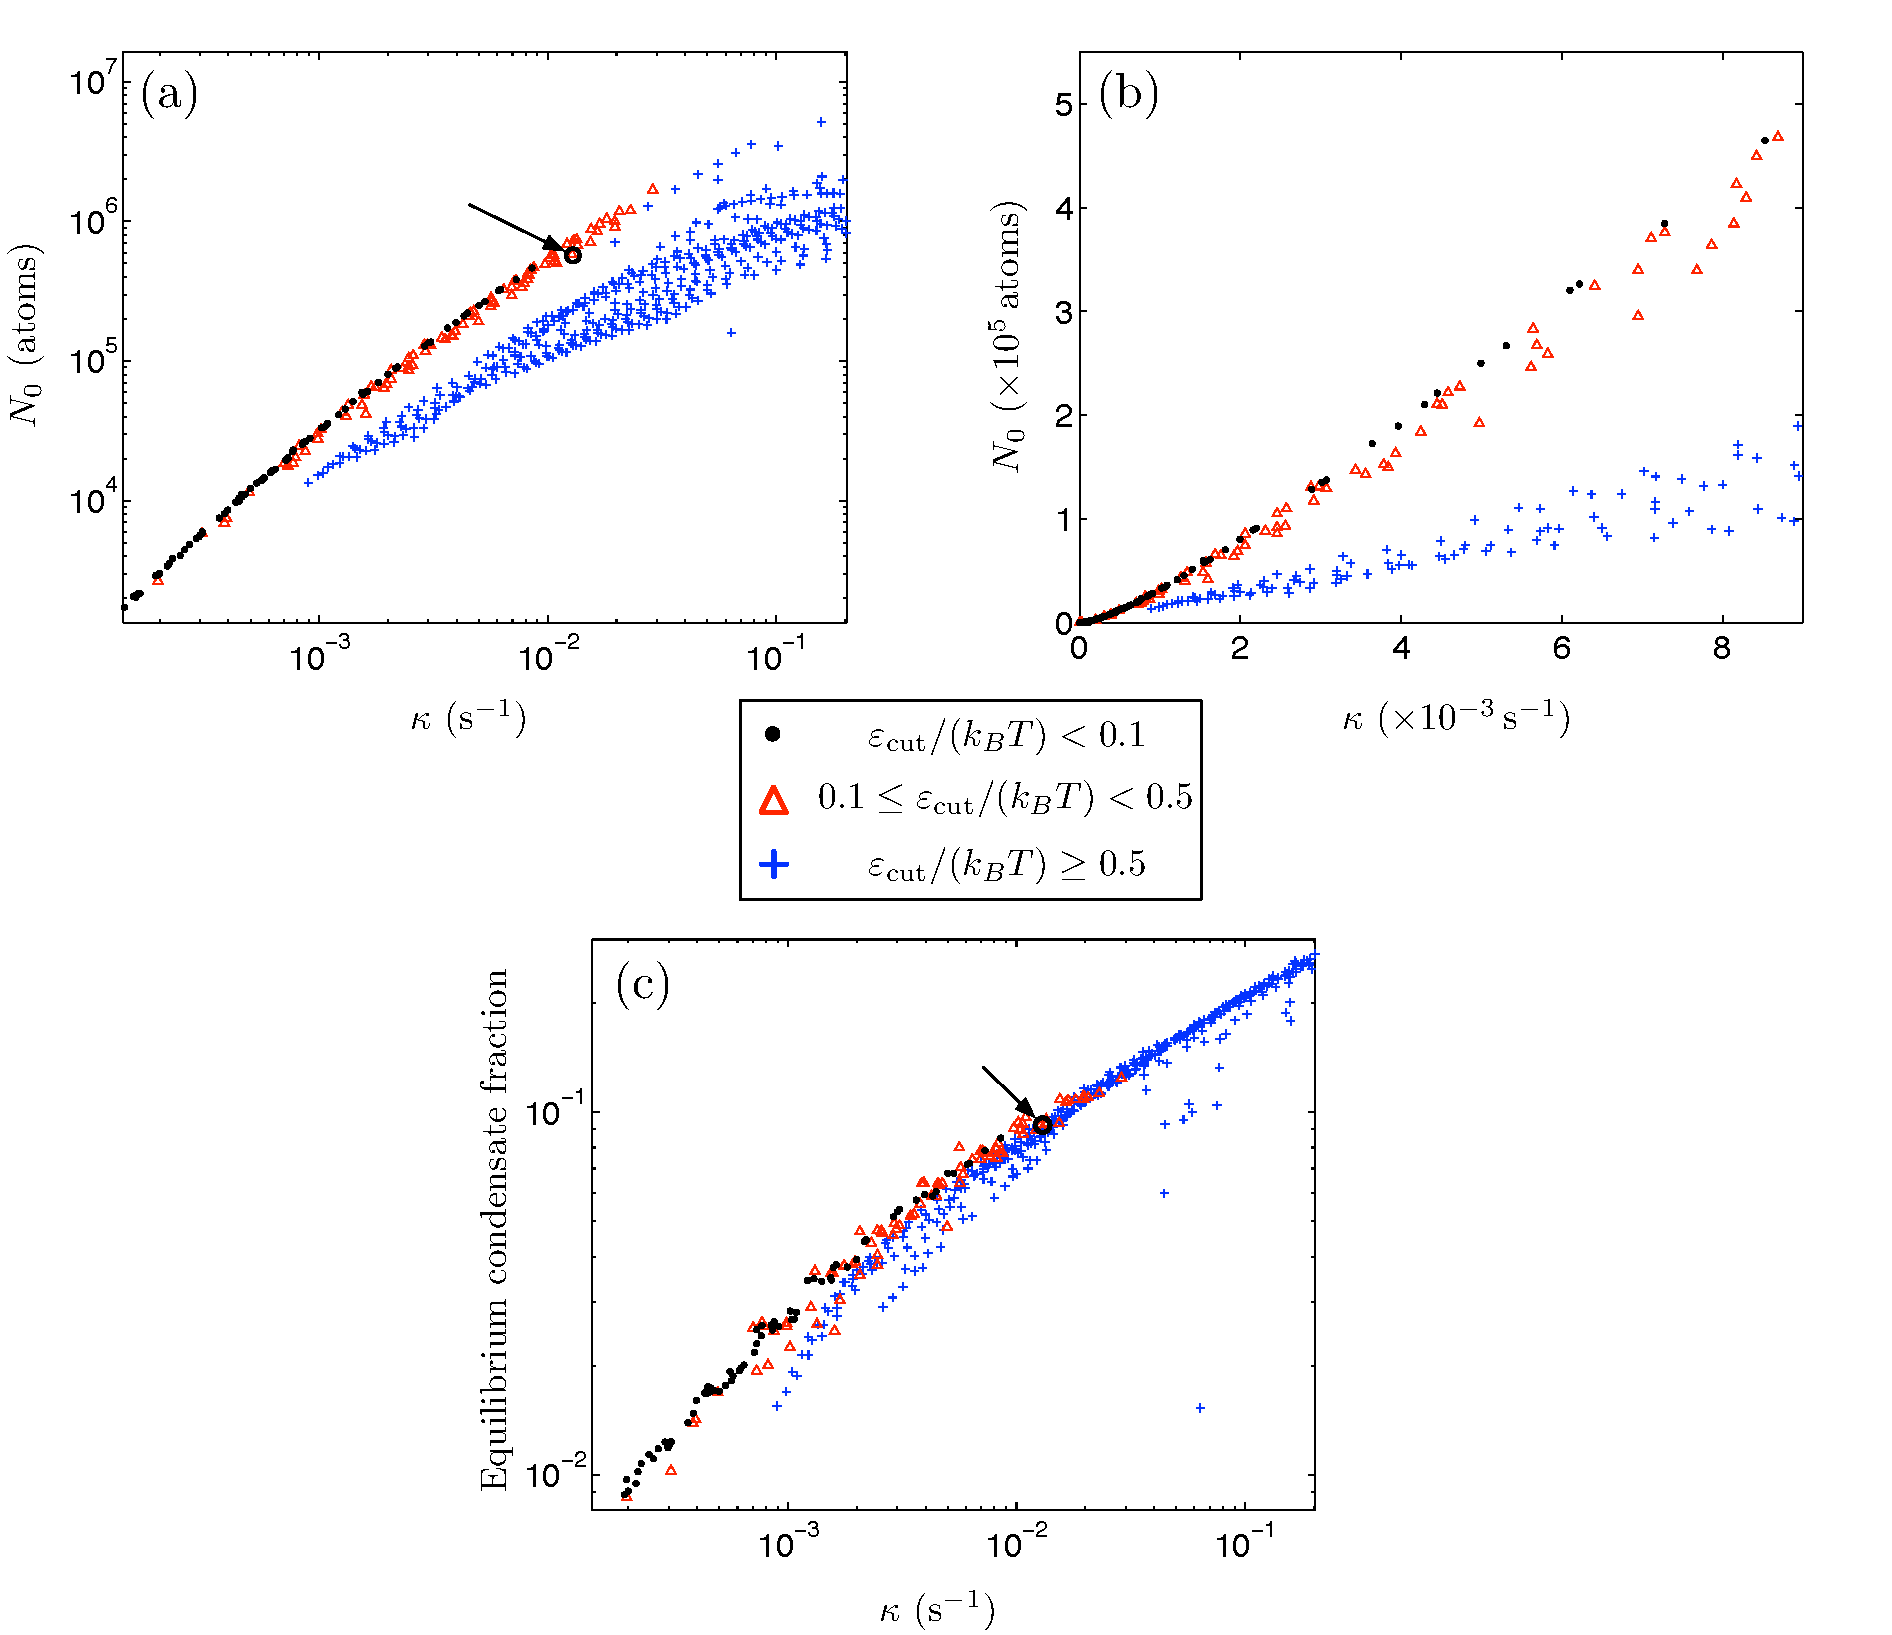
\includegraphics[width=15cm]{FigureOfMerit}
    \caption{Plot of equilibrium condensate properties as a function of the phase-space flux for the replenishment source $\kappa$. Figures (a) and (b) plot the equilibrium condensate number on different scales. Figure (c) plots the equilibrium condensate fraction $N_0/N$.  The results of the parameter scan are broken up into three groups (the black circles, red triangles and blue crosses) based on the extent to which the high-temperature limit discussed in this section applies to the results. The circled point with the arrow pointing to it corresponds to a simulation of the parameters for the last source in \tableref{KineticTheory:ExperimentalSources}, which has $\kappa= \unit[1.1\times 10^{-2}]{s\textsuperscript{-1}}$ (see main text).}
    \label{KineticTheory:FigureOfMerit}
\end{figure}

The results illustrated in \figureref{KineticTheory:FigureOfMerit} are separated into three groups based on the ratio $\varepsilon_\text{cut}/(k_B T)$.  The first group marked by black circles have $\varepsilon_\text{cut}/(k_B T) < 0.1$, and are the results for which the high-temperature limit can be considered to be a good approximation (satisfying the requirement $\varepsilon_\text{cut} \ll k_B T$) and $\kappa$ completely determines the properties of the replenishment source.  For this group of results, any equilibrium property of the system should appear to be a single (not necessarily straight) line when plotted as a function of $\kappa$.  The results in \figureref{KineticTheory:FigureOfMerit} demonstrate that these results can be viewed as a single function of $\kappa$.  The second group marked by red triangles have $0.1 \leq \varepsilon_\text{cut}/(k_B T) < 0.5$, and can be considered to be the results for which the high-temperature limit is almost a good approximation.  These results are reasonably close to the results of the first group, however there is a greater deviation for a given value of $\kappa$ indicating that the results can be almost seen as purely a function of $\kappa$. All remaining results fall into the third group for which $\varepsilon_\text{cut}/(k_B T) \geq 0.5$.  It can be seen that these points correspond to a broad range of equilibria for a given value of $\kappa$ indicating that the replenishment source cannot be described by $\kappa$ alone.
%  The origin of the distinct separation of the blue points from the red points in \figureref{KineticTheory:FigureOfMerit}(a) and \figureref{KineticTheory:FigureOfMerit}(b) is due to the use of a reduced sample of points in the three-dimensional parameter scan ($\Phi$, $T$, $\varepsilon_\text{cut}$) were used to limit the computational complexity of sampling a three-dimensional space spanning several orders of magnitude.

The first two panels of \figureref{KineticTheory:FigureOfMerit} both display the equilibrium condensate number as a function of the phase-space flux $\kappa$.  \figureref{KineticTheory:FigureOfMerit}(a) uses a log-log scale to highlight the behaviour for small and large values of $\kappa$, while \figureref{KineticTheory:FigureOfMerit}(b) uses a linear-linear scale to demonstrate that the black circles lying on a single line in (a) is not simply an artefact of plotting the results using a logarithmic scale.  Finally, \figureref{KineticTheory:FigureOfMerit}(c) displays the equilibrium condensate fraction as a function of $\kappa$.

\figureref{KineticTheory:FigureOfMerit}(a) and (b) demonstrate that it would be possible to produce atom lasers with respectable condensate numbers $N_0 \gtrsim 10^5$ (corresponding to atom laser fluxes of $\gtrsim\unit[3\times 10^4]{atoms/s}$ for the outcoupling rate $\gamma = \unit[0.3]{s\textsuperscript{-1}}$ chosen) by using replenishment sources that have a phase-space flux $\kappa \gtrsim \unit[10^{-3}]{s\textsuperscript{-1}}$.  To determine if this is experimentally feasible, the properties of a range of experimental atomic sources are detailed in \tableref{KineticTheory:ExperimentalSources} and the corresponding values of the phase-space flux $\kappa$ calculated.

\begin{table}
    \begin{minipage}{\textwidth}
        \renewcommand{\footnoterule}{}
        \centering
        \begin{tabular}{ p{3.563cm} c c c r}
        \toprule
         & Atomic flux   & Temperature  & Phase-space flux  &\\
        Atomic source &  $\Phi$  &  $T$ &  $\kappa$ &\\
        \midrule
        BECs in dipole traps & $\unit[10^5]{s\textsuperscript{-1}}$ ($\unit[55]{mHz}$)\footnote{This source is pulsed, and the flux is the mean flux over one cycle with the repetition rate listed in parentheses.}\footnote{This repetition rate it too low for this source to be useful (see main text). It is listed for purposes of comparison only.} & $<\unit[1]{\micro K}$ & $>\unit[1.9\times 10^{-3}]{s\textsuperscript{-1}}$ &~\citep{Chikkatur:2002qa} \\
        2D\textsuperscript{+}-MOT & $\unit[9\times 10^{9}]{s\textsuperscript{-1}}$ & $\unit[38]{mK}$\footnote{In keeping with the best-case scenario investigation being performed, this temperature assumes that the mean velocity of the atoms can be reduced to zero without affecting the distribution. This could be achieved, for example, by firing the source vertically below the main pumped atom laser experiment and taking the atoms from the mean turning point.}\footnote{The dominant contribution to this temperature is the spread in the longitudinal velocities of the atoms.} & $\unit[3 \times 10^{-12}]{s\textsuperscript{-1}}$ &~\citep{Dieckmann:1998} \\
        2D\textsuperscript{+}-MOT & $\unit[2\times 10^{10}]{s\textsuperscript{-1}}$ & $\unit[42]{mK}$\textsuperscript{\emph{cd}} & $\unit[5 \times 10^{-12}]{s\textsuperscript{-1}}$ &~\citep{Chaudhuri:2006} \\
        MM-MOT & $\unit[10^9]{s\textsuperscript{-1}}$ & $\unit[61]{\micro K}$\textsuperscript{\emph{c}} & $\unit[8 \times 10^{-5}]{s\textsuperscript{-1}}$ &~\citep{Cren:2002rt}\\
        LVIS & $\unit[5\times 10^{9}]{s\textsuperscript{-1}}$ & $\unit[25]{mK}$\textsuperscript{\emph{cd}} & $\unit[6 \times 10^{-12}]{s\textsuperscript{-1}}$ &~\citep{Lu:1996} \\
        Zeeman slower & $\unit[3.2\times 10^{12}]{s\textsuperscript{-1}}$ & $\unit[32]{mK}$\textsuperscript{\emph{cd}} & $\unit[2\times10^{-9}]{s\textsuperscript{-1}}$ &~\citep{Slowe:2005} \\
        Magnetic guide loaded from 3D-MOT & $\unit[7\times 10^{9}]{s\textsuperscript{-1}}$ & $\unit[400]{\micro K}$\textsuperscript{\emph{c}} & $\unit[2\times 10^{-6}]{s\textsuperscript{-1}}$ &~\citep{Lahaye:2004}\\
        3D-MOT loaded from Zeeman slower & $\unit[2\times 10^{10}]{s\textsuperscript{-1}}$ ($\unit[0.5]{Hz}$)\textsuperscript{\emph{a}} & $\unit[500]{\micro K}$ & $\unit[3\times 10^{-6}]{s\textsuperscript{-1}}$ &~\citep{Streed:2006}\\
        3D-MOT loaded from 2D\textsuperscript{+}-MOT & $\unit[3\times 10^8]{s\textsuperscript{-1}}$ ($\unit[3]{Hz}$)\textsuperscript{\emph{a}} & $\unit[8]{\micro K}$ & $\unit[1.1\times 10^{-2}]{s\textsuperscript{-1}}$ &~\citep{Muller:2007}\\
        \bottomrule
        \end{tabular}
    \end{minipage}
    \caption{Relevant properties of selected experimental cold atomic sources. The phase-space flux $\kappa$ is evaluated from the atomic flux and temperature values listed using \eqref{KineticTheory:KappaDefinition}.}
    \label{KineticTheory:ExperimentalSources}
\end{table}

The first source listed in \tableref{KineticTheory:ExperimentalSources} is the experiment by~\citet{Chikkatur:2002qa} that merged independently produced BECs in optical dipole traps that was discussed earlier.  This experiment is certainly not in the high-temperature limit, but it has been included for comparison purposes.  Of the remaining sources listed in \tableref{KineticTheory:ExperimentalSources}, most are many orders of magnitude away from being useful potential sources for a pumped atom laser (cf.~\figureref{KineticTheory:FigureOfMerit}).  The fluxes obtainable from these sources are insufficient to compensate for their higher temperatures. An increase of three-orders of magnitude in flux is necessary to compensate for an increase of a single order of magnitude in temperature [see \eqref{KineticTheory:KappaDefinition}].  Only the last atomic source satisfies the requirement $\kappa \gtrsim \unit[10^{-3}]{s\textsuperscript{-3}}$.  This experiment by~\citet{Muller:2007} is one of the sources in a dual atom interferometer designed for the precision measurement of accelerations and rotations~\citep{Muller:2009}.  A direct simulation has been performed for the parameters of this source, and the results are marked by a circle with an arrow pointing to it in \figureref{KineticTheory:FigureOfMerit}.  

The equilibrium condensate number for the source of~\citet{Muller:2007} is $N_0 = \unit[5 \times 10^5]{atoms}$, which would be a sufficiently large condensate to serve as a stable phase-reference for a produced atom laser were it a pure BEC.  However the equilibrium condensate fraction for this source is only 10\% [see \figureref{KineticTheory:FigureOfMerit}(c)].  With 90\% of the atoms in the thermal cloud, one cannot help but suspect that the significant thermal fluctuations would rule out the use of any atom laser produced by this source for interferometric use, which was our original motivation.  However, previous theoretical work investigating the transfer of statistics from a trapped (quasi-)condensate to an atom laser found that using high-momentum kick Raman outcoupling such as that proposed in the scheme presented here can filter some of these fluctuations causing the atom laser to have a larger coherence length than the condensate from which it was produced~\citep{Proukakis:2003}.  

It is not possible to investigate the transfer of statistics from the trapped component to the atom laser within the present model due to the simplifying assumption that it is only the condensate mode that is outcoupled to form the atom laser.  A more detailed three-dimensional model taking into account the full spatial dependence of the Raman outcoupling process would be necessary to fully determine the feasibility of using an atomic source such as that described by~\citet{Muller:2007} in the production of a truly continuous pumped atom laser.

%The equilibrium condensate number for the source of~\citet{Muller:2007} is $N_0 = \unit[5 \times 10^5]{atoms}$, which is a sufficiently large condensate to serve as a stable phase-reference for the produced atom laser.  However, the equilibrium condensate fraction is a mere 10\%.  This number is concerning as with 90\% of the atoms in the thermal cloud, it would be expected that there would be significant thermal fluctuations on any atom laser extracted.  Although the transfer of thermal fluctuations cannot be investigated in the kinetic model presented here, it seems reasonable to believe that thermal fluctuations would dominate the linewidth of the atom laser produced.  \figureref{KineticTheory:FigureOfMerit}(c) suggests that the situation won't be significantly improved if the atomic flux were increased by an order of magnitude. In this case with $\kappa \sim 10^{-1}$, the condensate fraction would have only increased to 20\%.  The temperature of the source cannot be reduced greatly either as at $T=\unit[8]{\micro K}$, it is not very far above the condensation temperature of the system of $T_c=\unit[1.2]{\micro K}$ for each $N=10^8$ atom pulse.



%Although this source is not quite in the high-temperature limit (the optimum evaporation cut-off is $\varepsilon_\text{cut} = 0.42 k_B T$)


\section{Conclusion}

The purpose of this chapter has been to investigate the feasibility of producing a continuously pumped atom laser driven by  collisions with a cloud of thermal atoms.  The method has been to investigate the best-case scenario in which the replenishment process introduces no heating to the trapped thermal component beyond that due to bringing the replenishing atoms into contact with the thermal cloud.  With these caveats in mind, the results are promising: using an existing experimental source~\citep{Muller:2007} it appears possible to produce steady-state condensates with large atom number ($\sim 5\times 10^5$ atoms) using the scheme presented in \sectionref{KineticTheory:Scheme}.  Should the atomic flux of this source be increased by an order of magnitude, the condensate number produced by this scheme could be pushed to $5\times 10^6$ atoms.  

Ultimately it is not the size of the condensate that we are interested in, but the flux of the atom laser produced and its coherence length.  The former goal will certainly be improved by larger equilibrium condensate sizes, however the atom laser itself will be useless unless its coherence length is sufficiently larger than that of cold thermal sources to offset its necessarily lower atom flux.  The model used in this chapter cannot answer the latter question.  To investigate this further it will be necessary to include the full multimode behaviour of the Raman outcoupler and the fluctuations of the thermal cloud.  This can be achieved through using a more general kinetic theory such as the `ZNG theory'~\citep{Zaremba:1999,Proukakis:2008} or the Stochastic Projected Gross-Pitaevskii equation (SPGPE)~\citep{Blakie:2008a}.

% One thing is certainly clear from the results presented here: the replenishment source for a collisionally-pumped atom laser must be close to degeneracy. It is simply not realistic to compensate for higher temperatures with a sufficiently increased flux.

% The author is cautiously optimistic about the promise of atom lasers replenished directly from thermal sources. Though this is not the only option for the production of a continuous atom laser.  Optical pumping, discussed in \chapterref{OpticalPumping} is another option, as is evaporation of an atomic beam in a magnetic guide~\citep{Mandonnet:2000lr,Lahaye:2004,Lahaye:2005uq}.


